\section{Grundlagen}

\subsection{MeSH}
\label{sec:mesh}
%Sinn und Bedeutung des MeSH wurden bereits in \autoref{sec:semedico} erläutert. 
In diesem Abschnitt wird die interne Struktur des MeSH beschrieben.

\subsubsection{MeSH Record Types}
%http://www.nlm.nih.gov/mesh/intro_record_types.html

\minisec{Descriptors}
Wie bereits in der Einleitung erwähnt, bildet der MeSH eine hierarchische Struktur, deren zentrales Element sogenannte Descriptors sind. Ein Descriptor ist die Repräsentation eines Begriffs bzw. eines Begriffsraumes für den im MeSH ein Index-Eintrag existiert. Descriptors haben eine teils mehr, teils weniger scharf abgegrenzte Bedeutung, je nach dem wie dies aus Sicht der Autoren des MeSH zur Zeit den Anforderungen des Wissenschaftbetriebs entspricht. Mehr Informationen zu den Organisationsprinzipien finden sich in \cite{MeSHOrgPrinciples2012}.\par

Neben den Descriptors gibt es zwei weitere sogenannte MeSH Record Types, die jedoch für diese Arbeit nicht von Interesse sind: Qualifiers und Supplementary Concept Records (SCR).\par

\minisec{Qualifiers}
Es existieren insgesamt 83 thematische Qualifiers. Sie erlauben es, im Zusammenspiel mit Descriptors, bestimmte Aspekte eines Themas sinnvoll zu gruppieren. Beispielsweise weist der Qualifier "`Liver/drug effects"' darauf hin, dass sich ein Artikel nicht allgemein mit der Leber, sondern mit den Auswirkungen von Medikamenten beschäftigt.

\minisec{Supplementary Concept Records}
Die Supplementary Concept Records (SCR) werden vor allem genutzt, um Chemikalien und Medikamente zu indizieren. Während sie grundsätzlich sehr ähnliche Attribute besitzen, besteht der wesentliche Unterschied zu Descriptors darin, dass SCRs keine Tree Numbers besitzen und sie folglich nicht selbst eine Hierarchie bilden. Stattdessen werden sie jeweils einem oder mehreren Descriptors zugeordnet und ergänzen bzw. spezifizieren so dessen Bedeutung. \par
%Es gibt mehr als 200\,000 SCR Einträge mit mehr als 500\,000 SCR terms.

\subsubsection{MeSH Komponenten und XML}
\label{sec:xml_struktur}
Der MeSH ist in zwei Formaten verfügbar: als XML-File sowie als ASCII-File. In dieser Arbeit wird die XML-Version verwendet, da zum einen die XML-Format reicher als die ASCII-Format ist \cite{Nelson2004}, und da zum anderen durch die Verwendung der seitens der NLM bereitgestellten dtd-Datei ein validiertes Parsen möglich ist. 

Nachfolgend werden die wichtigsten Begriffe im MeSH, nämlich Descriptor, Tree Number, Concept und Term für sich selbst und als XML-Element erklärt. \autoref{fig:MeSH_structure} zeigt den strukturellen Aufbau (der hier wichtigen Elemente) des MeSH. \par

Für eine detaillierte und vollständige Beschreibung aller XML-Elemente wird auf \cite{MeSHXML2012} verwiesen.\par

\begin{figure}[h]
\begin{center}
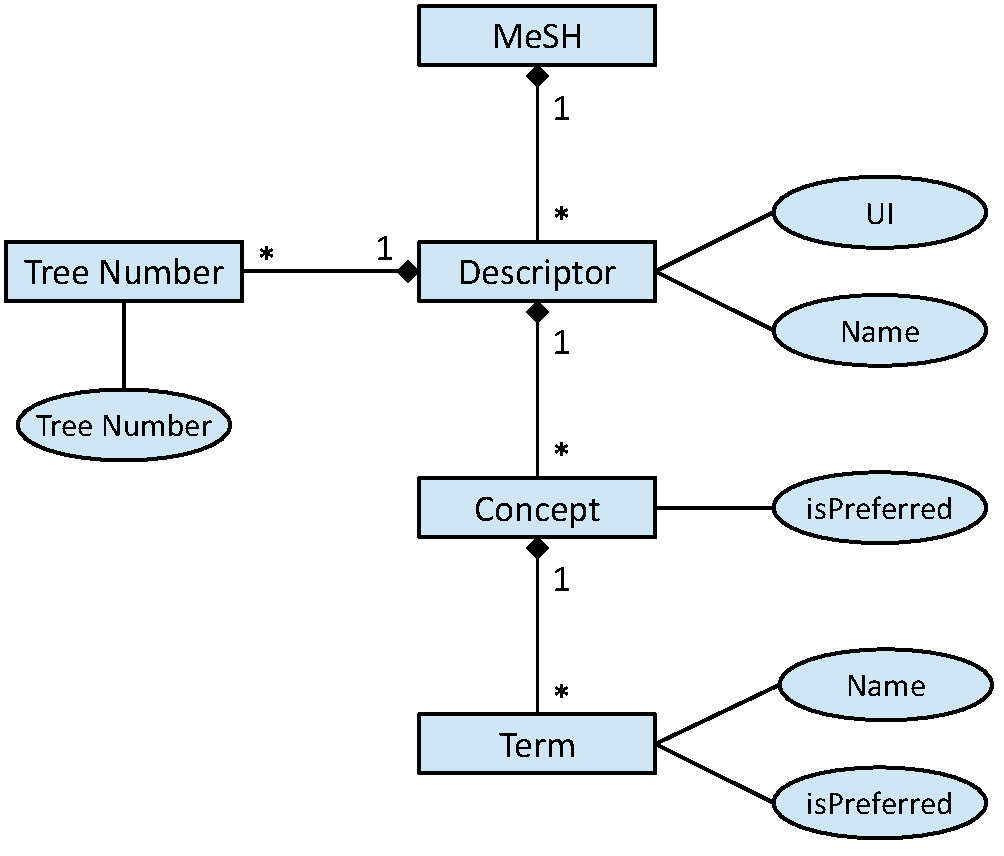
\includegraphics[width=0.8\textwidth]{figs/MeSH_structure_neu.pdf}
\end{center}
\caption{Datenstruktur des MeSH}
\label{fig:MeSH_structure}
\end{figure}

\minisec{MeSH}
Wenn man von SCRs absieht, besteht der MeSH aus einer Menge von Descriptors. Das entsprechende XML-Root-Element ist \code{<DescriptorRecordSet>}, welches alle Descriptors als direkte Kinder enthält.

\minisec{Descriptor}
Die Bedeutung der Descriptors wurde bereits weiter oben diskutiert.\par

Ein Descriptor als XML-Element ist ein \code{<DescriptorRecord>} und besteht, unter anderem, aus einer Menge von Tree Numbers (XML-Element: \code{<TreeNumberList>}) sowie aus einer Menge von Concepts (XML-Element: \code{<ConceptList>}). Tree Numbers betten Descriptors in eine oder mehrere Positionen in der Begriffshierarchie ein. Concepts erlauben eine feinere Einteilung der Bedeutung eines Descriptors.\par

Ein Descriptor kann eindeutig durch seine UI (XML-Element: \code{<DescriptorUI>}) und seinen Namen (XML-Element \code{<DescriptorName>}) identifiziert werden. Der Name ist dabei der  \code{<PreferredName>} des \code{<PrefferedConcepts>} des Descriptors.\par

Es sind keine expliziten Relationen, wie zum Beispiel Inklusion auf Descriptors, definiert. Siehe dazu auch den Abschnitt unten zu Tree Numbers. \par

Ein Descriptor wird auch als Descriptor Record oder Main Heading bezeichnet.

\minisec{Concept}
Ein Concept besteht aus einer Menge von Terms und kann über seine ID (XML-Element \code{<ConceptUI>}) eindeutig identifiziert werden. \par

Ein Concept beschreibt eine begriffliche Untereinheit eines Descriptors. Alle Terme innerhalb eines Concepts sind synonym zueinander. \par

\minisec{Tree Number}
Eine Tree Number ist eine alpha-numerische Zeichenkette und verweist an einer bestimmte Position des MeSH auf den Descriptor, der diese Tree Number enthält. Das dazugehörige XML-Element ist  \code{<TreeNumber>}. \par
% Beispiel:
% \begin{verbatim}
% <TreeNumber>C02.839.040</TreeNumber>
% \end{verbatim}
Es ist an dieser Stelle zu bemerken, dass die hierarchische Struktur des MeSH nicht explizit als XML-Element vorliegt. Vielmehr ergibt sich die Struktur allein implizit durch die Namensgebung der Tree Numbers, also eben aus der Eigenschaft, dass eine Tree Number $x.y.z$ dafür steht, dass die Tree Number $x.y$ der Vater der Tree Number $x.y.z$ ist. \par

Diese Verflechtung von ID einer Tree Number und Strukturinformation ist aus unserer Sicht nicht wünschenswert: Unter Aufrechterhaltung dieser Eigenschaft führt ein lokales Verändern der hierarchischen Struktur zu nicht-lokalen Änderungen der Tree Number. Beispielsweise führt ein Verschieben einer Tree Number dazu, dass auch alle untergeordneten Tree Numbers umbenannt werden. Das macht ein Arbeiten mit der Hierarchie unnötig kompliziert. In \autoref{sec:repräsentation_des_mesh_als_baum} wird eine Möglichkeit diskutiert, wie diese Verflechtung beseitigt werden kann. \par

\minisec{Term}
Ein Term wird auch als Entry Term bezeichnet. Und \cite{MeSHEntryTerms2012} beschreibt Entry Terms folgendermaßen:
\begin{quotation}
"`Entry terms, sometimes called "`See cross-references"' in printed listings, are synonyms, alternate forms, and other closely related terms in a given MeSH record that are generally used interchangeably with the preferred term for the purposes of indexing and retrieval, thus increasing the access points to MeSH-indexed data."'
\end{quotation}

Das dazugehörige XML-Element ist  \code{<Term>}. 

%\subsubsection {MeSH Struktur}
%MeSH-Descriptors sind, indirekt über ihre Tree Numbers, in 16 Bäumen angeordnet. Die Wurzeln der Bäume werden auch Kategorien genannt und bezeichnen grundlegende Konzepte, wie beispielsweise "`A (Anatomy)"' oder "`B (Organisms)"'. Diese Wurzeln sind allerdings nicht als Descriptor im MeSH repräsentiert. Jede Kategorie besitzt Unterkategorien, etwa "`A01 (Body Regions)"', in welchen die Tree Numbers der Descriptors angeordnet sind. Je tiefer eine Tree Number dabei in einem Baum liegt, desto spezieller ist die Bedeutung des dazugehörigen Descriptors im Kontext des Astes, in dem die Tree Number liegt. Siehe dazu auch \autoref{fig:MeSH_structure}.

\subsubsection{Jährliche Änderungen}
\label{sec:anual_changes}
Jedes Jahr erscheint eine neue, an die aktuellen Entwicklungen der Wissenschaft angepasste Version des MeSH. Auch für Semedico soll die jeweils aktuelle Version des MeSH als Datengrundlage verwendet werden. Dazu wird, wie zuvor in \autoref{sec:MeSH_erstellen} erklärt, eine Folge von Operationen auf den MeSH angewandt, um daraus den Semedico-MeSH zu erzeugen. Problematisch ist hierbei, dass mit jeder Änderung am MeSH die Operationen zur Erzeugung des Semedico-MeSH potentiell unmöglich werden. Beispielsweise kann eine Tree Vertex nicht mehr verschoben werden, falls sie in der neuen Version des MeSH nicht mehr existiert.\par

\minisec{Lösungsmöglichkeiten}

\begin{figure}
\begin{center}
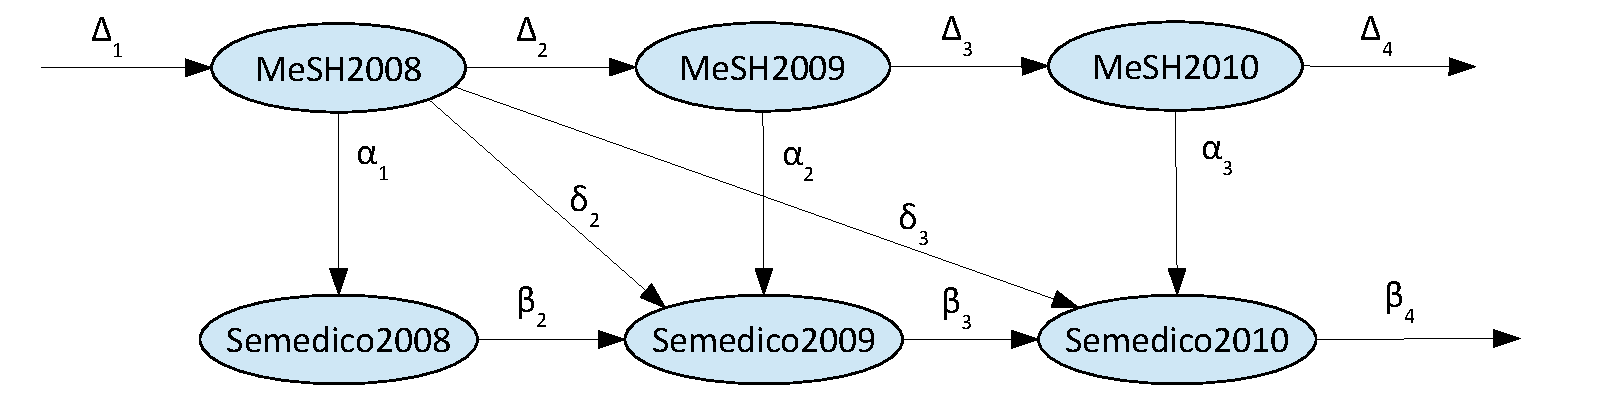
\includegraphics[width=0.9\textwidth]{figs/anualChangesConcepts.pdf}
\end{center}
\caption{Möglichkeiten zur Erzeugung des jährlichen Semedico-MeSH}
\label{fig:anualChangesConcept}
\end{figure}

\autoref{fig:anualChangesConcept} zeigt schematisch die Lösungsvarianten, die nachfolgend konzeptionell erläutert werden. \par

Gegeben sind \code{MeSH2008} sowie \code{Semedico2008}, also der MeSH des Jahres 2008 und der darauf basierende Semedico-MeSH. Daraus kann $\alpha_1$ bestimmt werden und ist damit ebenfalls gegeben. $\Delta_i$, $\alpha_i$, $\beta_i$, $\delta_i$ seien Operationsfolgen, die einzelne Versionen des MeSH, wie in \autoref{fig:anualChangesConcept} dargestellt, ineinander überführen. Ziel ist es, den Semedico-MeSH für die Folgejahre zu erstellen. Um das zu erreichen, gibt es wenigstens drei Möglichkeiten:
\begin{itemize}
  \item[$(\alpha)$] Den MeSH des aktuellen Jahres in den Semedico-MeSH überführen. Dazu wird $\alpha_i$ als Aktualisierung von $\alpha_{i-1}$ unter Zuhilfenahme von $\Delta_i$ erstellt.
  \item[$(\beta)$] Den Semedico-MeSH des vorangegangen Jahres aktualisieren. Hierzu wird $\beta_i$ als modifizierte Teilmenge von $\Delta_i$ erstellt - als Menge all der Operationen aus $\Delta_i$ die auf \code{Semedico20xx} angewandt werden können. 
  \item[$(\delta)$] Direkt aus dem MeSH2008 den aktuellen Semedico-MeSH erzeugen. Dafür wird $\delta_i$ als Vereinigung von $\delta_{i-1}$ und $\Delta_i$ erzeugt.
\end{itemize}

Für diese Studienarbeit wurde die erste Variante $(\alpha)$ umgesetzt. Zum einen werden also die jährlichen Änderungen $(\Delta)$ des MeSHs benötigt. In \autoref{sec:vergleichBaume} \textit{\nameref{sec:vergleichBaume}} wird beschrieben wie diese ermittelt werden. Zum anderen muss $\alpha$ aktualisiert werden. Das Vorgehen dazu ist in \autoref{sec:merging} \textit{\nameref{sec:merging}} erklärt. Als Basis werden hier in den restlichen Unterabschnitten dieses Abschnitts grundlegende Begriffe der Graphentheorie, eine Formalisierung des MeSH, sowie verschiedene Operationen und Relationen auf dem formalisierten MeSH eingeführt.

\minisec{Änderungen verfolgen} 
Online sind für die jeweils aktuelle Version Änderungslisten verfügbar. Allerdings sind diese weder umfassend noch vollständig\footnote{See "`4. MeSH Vocabulary Changes for 2013"' of \url{http://www.nlm.nih.gov/mesh/introduction.html}}. Das heißt sie enthalten nicht alle Informationen zu den Änderungen. Beispielsweise gibt es keine Informationen dazu \textit{welche} Attribute eines Descriptors geändert wurde, sondern nur, \textit{dass} er geändert wurde. Und sie enthalten auch nicht alle Änderungen. Beispielsweise gibt es überhaupt keine Informationen zu Aufteilungen von Descriptors. \par

Daher ist es notwendig eigene Methoden zu entwickeln, um diese Änderungen zu bestimmen. Siehe dazu \autoref{sec:vergleichBaume} \textit{\nameref{sec:vergleichBaume}}. 

\subsection{Graphentheorie}
Dieser Abschnitt definiert die klassischen Begriffe der Graphentheorie. Sie sind in wesentlichen Teilen~\cite{Diestel2010} entnommen.

\begin{definition}[Graph, Knoten, Kante]
%Ein Graph $G$ ist ein 2-Tupel $(V,E)$ mit $E \subseteq V \times V$. Die Elemente der Menge $V$ werden Knoten genannt. Die Elemente der Menge $E$ werden Kanten genannt. Sie sind geordnete Paare aus Elementen $V$s. 
Ein Graph $G$ ist ein 2-Tupel $(V,E)$ mit $E \subseteq V^2$. Die Elemente der Menge $V$ werden Knoten genannt. Die Elemente der Menge $E$ werden Kanten genannt. Ist $\{x,y\} \in E$, so bezeichnen wir diese Kante auch mit $xy$.
\end{definition}

\begin{definition}[Knotenmenge, Kantenmenge]
Sei $G=(W,F)$ ein Graph. Wir bezeichnen dann $E(G) = F$ als Kantenmenge und $V(G) = W$ als Knotenmenge $G$s.
% \begin{itemize}
%   \item[]$E(G) = W$ als Knotenmenge
%   \item[]$V(G) = F$ als Kantenmenge
% \end{itemize}
\end{definition}

\begin{definition}[Teilgraph]
Ein Graph $S$ heißt Teilgraph eines Graphen $G$ genau dann, wenn gilt
\[ 
 E(S) \subseteq E(G) \wedge V(S) \subseteq V(G)
\]
\end{definition}

\begin{definition}[Pfad, Zyklus, Kreis]
Ein Pfad $P$ in einem Graphen $G$ ist eine Folge von Knoten $(x_0,\ldots,x_k)$, so dass:
\begin{align*}
	\forall (i=0,\ldots,k-1) : x_ix_{i+1} \in E(G)  
\end{align*}

Die Länge des Pfades $P$ ist gleich $k-1$ und wird mit $l(P)$ bezeichnet.\par

Sei $s=x_0$ und $t=x_k$. Dann heißt $P$ auch $s-t$-Pfad.\par

Existieren $m,n \in \{0,\ldots,k\}$ so dass $x_m = x_n$, dann heißt $P$ Zyklus. \par

%Gelten $k>0$ und $x_0 = x_k$ und sind sonst alle $x_i$ verschieden, so heißt $P$ Kreis. \par
Gilt $x_0 = x_k$ und sind sonst alle $x_i$ verschieden, so heißt $P$ Kreis. \par
\end{definition}

\begin{definition}[Zusammenhängend]
Ein nicht leerer Graph heißt zusammenhängend, wenn er für je zwei seiner Knoten $x$ und $y$ einen $x-y$-Pfad enthält. 
\end{definition}

\begin{definition}[Baum, Wurzel]
Ein Graph $G$ heißt Baum, falls er zusammenhängend ist und es kein $S \subseteq V(G)$ mit $l(S) > 1$  gibt, so dass $S$ ein Kreis in $G$ ist.\par

In einem Baum $G$ gibt es einen beliebigen aber ausgezeichneten Knoten aus $V(G)$, der Wurzel genannt wird. Wir schreiben dafür auch $root(G)$.
\end{definition}

\begin{definition} [Tiefe eines Knotens]
Sei $G$ ein Baum und $v \in V(G)$. Sei weiter $P$ ein $root(G)-v$-Pfad. Dann setzen wir die Tiefe $v$s als $d(v) = l(P)$.  
\end{definition}

\begin{definition}[Verwandtschaft]
Zwei Knoten $x,y$ eines Baumes $G$ heißen benachbart oder adjazent, falls $xy \in E(G)$ gilt. \par

In einem Baum $G$ heißt ein Knoten $x$ Vater eines Knoten $y$ und der Knoten $y$ heißt Kind des Knotens $x$, falls gilt: 
\[ xy \in E(G) \wedge d(x) < d(y) \]

Die Menge aller Kinder eines Knoten $x$ wird auch als $children(x)$ und der Vater eines Knotens $x$ auch als $dad(x)$ bezeichnet. \par

In einem Baum $G$ heißt ein Knoten $x$ Vorfahre eines Knoten $y$ und der Knoten $y$ heißt Nachkomme des Knotens $x$ falls ein $x-y$-Pfad in $G$ existiert und $d(x) < d(y)$ gilt.
\end{definition}

\begin{definition}[Label und Typ]
 Ein Label besteht aus einem textuellem Schlüssel und einem beliebigen Wert, und wird einem Knoten oder einer Kante zugeordnet. \par

 Die Menge der Schlüssel der Label eines Knoten $v$ bzw. einer Kante $k$ wird als $label(v)$ bzw. $label(k)$ bezeichnet. \par 

 Den Wert eines Labels $l$ eines Knotens $v$ bzw. einer Kante $k$ identifizieren wir mit $v.l$ bzw. $k.l$. Ist der Wert von $l$ leer, so sagen wir auch $v$ bzw. $k$ sind vom Typ $l$. \par

 Ein Label erlaubt es damit Knoten und Kanten beliebige Zusatzinformationen zuzuordnen.
\end{definition}

% \minisec{Definitionen von \ldots }
% \begin{itemize}
%   \item Graph: gerichtet, ungerichtet
%   \item Vater, Mutter, Kind, Vorfahre, Nachkomme
%   \item Pfad
%   \item Baum
%   \item Wurzelknoten
%   \item Tiefe eines Knotens
% \end{itemize}


\subsection{Der MeSH als Graph}
\label{sec:repräsentation_des_mesh_als_baum}
%Ein MeSH wird in nachfolgend beschriebender Weise als Graph formalisiert. \par
Gegeben sei ein MeSH $M$. Dieser wird, wie nachfolgend beschrieben, als \textit{MeSH-Graph} $G_M$ formalisiert: 

\begin{itemize}
 \item Jeder Descriptor $d$ aus $M$ wird durch einen Knoten $v_d$ vom Typ \code{Descriptor} in $G_M$ repräsentiert. $v_d$ erhält zwei Label \code{name} und \code{ui} deren Werte der Name bzw. die UI von $d$ sind.
 \item Jede Tree Number $t$ aus $M$ wird durch einen Knoten $v_t$ vom Typ \code{TreeVertex} in $G_M$ repräsentiert. $v_t$ erhält ein Label \code{name} dessen Wert die tatsächliche Tree Number $t$ s ist. Weiterhin erhält $G_M$ eine Kante vom Typ \code{Descriptor} von $v_t$ nach $v_d$, wobei $v_d$ der Knoten ist durch den der Descriptor von $t$ repräsentiert wird.
 \item Für jedes Paar Tree Numbers $s$ und $t$ aus $M$, für die $s$ eine direkte Unterkategorie von $t$ ist, enthält $G_M$ eine Kante des Typs \code{TreeVertex} von $\{v_s,v_t\}$. \\ $s$ ist eine direkte Unterkategorie von $t$ wenn die Tree Number von $s$ sich als nachfolgende Konkatenation schreiben lässt. Sei dazu $tnr$ die Tree Number von $t$: \[tnr.[0123456789]^*\] \par
 \item $G_M$ erhält einen ausgezeichneten Knoten \code{r} vom Typ \code{TreeVertex}.
 \item Für jede Tree Number $t$ die keinen Punkt enthält, gibt es in $G_M$ eine Kante $\{r,t\}$ vom Typ \code{TreeVertex}.
\end{itemize}

Vereinfacht gesagt werden Descriptors und Tree Numbers als Knoten, und die Strukturinformation der Tree Numbers (d.h. der Wert ihrer Tree Number und welcher der dazugehörige Descriptor ist) als Kanten angeordnet. Damit ist $G_M$ eine vollständige Repräsentation von $M$ und es ergeben sich - entsprechend der Typen der Kanten und Knoten - zwei interessante Graphen wie folgt:

\minisec{Baum der Tree Vertices}
Abgesehen vom Wurzelknoten wird jede Tree Number des MeSH durch genau einen Knoten (des Typs \code{TreeVertex}) repräsentiert, und umgekehrt. Ebenso wird die Hierarchieinformation jeder Tree Number durch genau eine Kante (des Typs \code{TreeVertex}) repräsentiert, und umgekehrt. Da Tree Numbers per Definition höchstens einen Vater besitzen, ist die Menge aller Kanten und Knoten vom Typ \code{TreeVertex} mit Knoten \code{r} als Wurzel ein Baum und ein Teilgraph von $G_M$. \par
\textit{Wenn nachfolgend vom \textit{MeSH-Tree} bzw. verkürzt \textit{Tree} gesprochen wird, ist dieser Baum gemeint. Ebenso meinen wir nachfolgend mit \textit{Descriptor} und \textit{Tree Vertex} im Allgemeinen einen Knoten vom Typ \code{Descriptor} bzw. \code{TreeVertex}.}

\minisec{Polyhierarchie der Descriptors}
Parallel dazu existiert eine Polyhierarchie aus Descriptors: Jeder Tree Number ist genau ein Descriptor zugeordnet und über den MeSH-Tree stehen auch diese Descriptors untereinander in hierarchischer Beziehung. Während allerdings eine Tree Number genau einem Knoten im MeSH-Tree zugeordnet ist, besitzt ein Descriptor so viele Kanten in $G_M$, wie er Tree Numbers besitzt. Anschaulich gesprochen entsteht die Polyhierarchie der Descriptors aus $G_M$, indem alle Knoten eines jeden Descriptors zu einem einzigen vereint. Der entstehende Graph ist im Allgemeinen kein Baum. \par
Diese Polyhierarchie ist eine vereinfachte Repräsentation des MeSH, da hier ein wesentlicher Teil der Hierachie verloren gehen: die genaue Beziehung der Tree Numbers untereinander. Erhalten bleibt nur die Hierarchie auf Descriptor-Ebene. \par

%[TODO: bild, formalere Beschreibung der Polyhierarchie?] \par
%Siehe dazu auch \autoref{fig:polyhierachie}.\todo{figure} 

% Wie in \autoref{sec:xml_struktur} beschrieben und in Bild TODO veranschaulicht, setzt sich der MeSH aus Descriptors und ein Descriptor aus einer Reihe von Tree
% Numbers zusammen, welche ihrerseits zu jeweils genau einem Descriptor gehören. Die Gesamtheit der Tree Numbers ergibt dabei die hierarchische Struktur des MeSH.

%Dieser Wald, bestehend aus allen 16 Bäumen, ist eine vollständige Repräsentation der Descriptors des MeSH, da jeder Descriptor wenigstens eine Tree Number besitzt und daher enthalten ist. Zudem ist diese Repräsentationsform ist natürlich, da sich die Struktur des MeSH unmittelbar in der Struktur des Waldes wiedergespiegelt: Knoten repräsentieren die textuellen Informationen des MeSH (z.B. Concepts und Terms), während Kanten die Strukturinformation der Tree Numbers kodieren.
% Zudem können bei Bedarf alle Methoden und Konzepte der Graphentheorie angewandt werden. \par
%Ein weiterer Vorteil der Repräsentation als Graph liegt darin, dass die strukturelle Information nun durch die Struktur des Graphen kodiert ist und d
%Wie dargestellt, können Tree Numbers als ID ihrer Knoten im Baum angesehen werden. Anstelle von Tree Numbers sprechen wir deshalb fortan von Tree Vertices, welche als eindeutige ID ein Label \code{name} besitzen, dessen Wert die Tree Number ist. \par

%Wenn wir fortan vom \textit{MeSH-Tree} bzw. verkürzt vom \textit{Tree} sprechen, dann ist damit der Baum gemeint, der sich ergibt, wenn man alle \textit{Unter}kategorien der 16 Bäume unmittelbar einer gemeinsamen Wurzel unterordnet.\par

\subsubsection{Operationen und Transformationen}
\label{sec:mesh_operationen}

Es folgt eine Auflistung von Definitionen zu Operationen auf MeSH-Graphen. Sei $\textrm{MeSH}$ die Menge aller MeSH-Graphen. Eine MeSH-Operation $o$ ist Operation der Form
% und seien $G_1$, $G_2 \in \textrm{MeSH}$ zwei Mesh-Graphen, sowie $T_1$, $T_2$ die dazugehörigen Mesh-Trees entsprechend \autoref{sec:repräsentation_des_mesh_als_baum}. \par

\[
o: MeSH \times Param \rightarrow MeSH 
\] % : G_1 \mapsto G_2\]

wobei $Param$ die Menge der Parameter der Operation $o$ darstellt. \par

Das Fixieren der Parameter $Param$ einer konkreten Operation $o$, bildet $o$ auf die \textit{Transformation} $t_o$ ab. $t_o$ ist folglich eine innere unäre Operation über $\textrm{MeSH}$.\par

Eine Folge von Transformationen ist eine Menge von Transformationen mit einer totalen Ordnung. Die Anwendung einer Transformationsfolge $T$ auf einen MeSH-Graphen $G$ bedeutet die sequentielle Anwendung aller Transformationen aus $T$ auf $G$ entsprechend ihrer Ordnung. \par

%Dann ist eine MesH-Operation eine Abbildung $o: MeSH \times\rightarrow MeSH : G_M \mapsto G_M'$

Nachfolgend beschreiben wir Operationen auf MeSH-Graphen. Sie sind in dem Sinne atomar, als das sie alle grundlegenden Operationen beschreiben, die wir im Kontext das MeSH als \textit{eine} Operation ansehen. Beispielsweise zwar kann ein Vertex-Verschieben durch eine Kombination von Vertex-Löschung und Vertex-Addition realisiert werden. Allerdings würde ein Verschieben dann mehr als eine Operation benötigen. Das ist zu vermeiden, da wir in \autoref{sec:vergleichBaume} möglichst kurze Transformationsfolgen suchen und folglich eine einheitliche Länge für jede elementare Operation voraussetzen.\par

Sei nachfolgend $G_M \in \textrm{MeSH}$ und $T_M$ der zu $G_M$ gehörende MeSH-Tree, entsprechend \autoref{sec:repräsentation_des_mesh_als_baum}.\par

% d.\,h. manche Operationen lassen sich als Kombination anderer Operationen darstellen. Sie sind aber in dem Sinne elementar, als das wir alle Operationen auflisten, die wir im Kontext des MeSH unterscheiden können müssen. In \autoref{sec:vergleichBaume} versuchen wir Transformationsfolgen zu erhalten. Dies ist grundsätzlich nicht eindeutig möglich. Folglich verwenden wir heuristische Methoden um ein möglichst gutes Ergebnis zu erzielen. Und diese Heuristiken arbeiten umso besser, umso Dazu ist es 

%Hinzufügen einer Tree Vertex
%\begin{definition}[\code{vertexAdd(name, parent, desc)}]
\begin{definition}[Vertex-Addition]

Schreibweise: \code{vertexAdd(name, parent, desc)} \par

Fügt im $T_M$ eine Tree Vertex $v$ mit Namen \code{name} als Kind der Tree Vertex \code{parent} ein. Diese Tree Vertex wird dabei dem Descriptor \code{desc} zugeordnet, d.\,h. in $G_M$ wird eine Kante vom Typ \code{Descriptor} von $v$ zu \code{desc} eingefügt. \par

Verkürzte Schreibweise: \code{vertexAdd(loc, desc)}, wobei \code{loc} gerade das Paar aus \code{name} und \code{parent} ist.
\end{definition}

%Löschen einer Tree Vertex:
%\begin{definition}[\code{vertexDel(vertex, rec)}]
\begin{definition}[Vertex-Löschung]
Schreibweise: \code{vertexDel(vertex, rec)} \par
Wenn \code{rec = true} werden \code{vertex} und auch alle Nachkommen von \code{vertex} aus $T_M$ entfernt. Ansonsten wird nur \code{vertex} entfernt. Ebenso werden alle Kanten der Form $\{vertex,v\}$ mit $v \in V(G_M)$ entfernt.

%Wenn \code{vertex} Kinder hatte, besitzen diese danach keinen Vater mehr. \par
\end{definition}

%Verschieben einer Tree Vertex:
%\begin{definition}[\code{vertexMove(v, oldParent, newParent, oldDesc, newDesc)}
\begin{definition}[Vertex-Verschiebung]
Schreibweise: \code{vertexMove(v, oldParent, newParent, oldDesc, newDesc)} \par

Verschiebt eine Tree Vertex \code{v}, so dass \code{newParent} der Vater von \code{v} in in $T_M$ und \code{newDesc} der zu \code{v} gebundene Descriptor ist. Der bisherige Vater von \code{vertex} ist \code{oldParent}, und der bisher zu \code{v} gebundene Descriptor ist \code{oldDesc}. 
\end{definition}
Damit ist ein Verschieben ein Umhängen von Kanten und folglich werden Tree-Vertices innerhalb eines MeSH-Trees immer mitsamt all ihrer Kinder verschoben. Außerdem müssen sich nicht Descriptor \textit{und} Vater von \code{v} ändern. Wird nur der zu \code{v} gehörende Descriptor verändert, so nennen wir das als Spezialfall dieser Operation auch Vertex-Neuverknüpfung oder Vertex-Rebinding.

% %Rebdinding einer Tree Vertex
% \begin{definition}[\code{vertexReb(vertex, oldDesc, newDesc)}]
% Verändert die der Tree Vertex \code{vertex} zugeordneten Descriptor nach \code{newDesc}.
% \end{definition}

%Umbenennen einer Tree Vertex
%\begin{definition}[\code{vertexRen(vertex, newName)}]
\begin{definition}[Vertex-Umbenennung]
Schreibweise: \code{vertexRen(vertex, newName)} \par

Verändert den Wert des Labels \code{name} der Tree-Vertex \code{vertex} zu \code{newName}.
\end{definition}

%Hinzufügen eines Descriptors
%\begin{definition}[\code{descAdd(desc, locs)}]
\begin{definition}[Descriptor-Addition]
Schreibweise: \code{descAdd(desc, locs)} \par

Fügt den Descriptor \code{desc} hinzu. Dem Descriptor sind eine Menge von Tree Vertices zugeordnet, die ebenfalls hinzugefügt werden. Ihr Name und Position wird durch \code{locs} beschrieben. \code{locs} besteht aus Paaren von \code{name} und \code{parentVertex}, wobei \code{name} der Name der Tree Vertex und \code{parentVertex} der Vater dieser Tree Vertex ist.
\end{definition}

%Löschen eines Descriptors
\begin{definition}[Descriptor-Löschung]
Schreibweise: \code{descDel(desc)} \par

Löscht den Descriptor \code{desc}. Löscht auch alle zu \code{desc} gehörigen Tree Vertices sowie entsprechend sonst verwaiste Kanten.
\end{definition}

%Relabelling eines Descriptors:
%\begin{definition}[\code{descRel(desc, newName)}]
\begin{definition}[Descriptor-Relabelling]
Schreibweise: \code{descRel(desc, newName)} \par

Ändert den Wert des Labels \code{name} des Descriptors \code{desc} nach \code{newName}.
\end{definition}

%Renaming eines Descriptors
%\begin{definition}[\code{descRen(desc, newUI)}]
\begin{definition}[Descriptor-Umbenennung]
Schreibweise: \code{descRen(desc, newUI)} \par

Ändert den Wert des Labels \code{ui} des Descriptors \code{desc} nach \code{newUI}.
\end{definition}

\subsubsection{Kommutativität von Kompositionen der Transformationen}
\label{sec:trans_prop}
Die im vorigen Abschnitt definierten Transformationen lassen sich in folgende Gruppen einteilen:
\begin{enumerate}
 \item[(1)] Transformationen die ausschließlich Knoten und Kanten hinzufügen: Vertex-Addition und Descriptor-Addition. 
 \item[(2)] Transformationen die ausschließlich Knoten und Kanten löschen: Vertex-Löschung und Descriptor-Löschung
 \item[(3)] Transformationen die ausschließlich Labels ändern: Vertex-Umbenennung, Descriptor-Relabelling und Descriptor-Umbenennung
 \item[(4)] Vertex-Verschiebungen
\end{enumerate}

Kompositionen von Transformationen der ersten Gruppe sind kommutativ, denn die Komposition von Hinzufügen von Knoten oder Kanten ist kommutativ, da die Komposition von Vereinigungen von Mengen kommutativ ist. Analog zur ersten Gruppe sind auch Kompositionen der Transformationen der zweiten Gruppe kommutativ.\par

Kompositionen von Transformationen der dritten Gruppe sind im Allgemeinen nicht kommutativ: Beispielsweise ist das Ergebnis verschieden, je nachdem ob man die UI eines Descriptors erst in \code{001} und dann in \code{002} ändert, oder umgekehrt. Allerdings lässt sich jede solche nicht kommutative Komposition trivial als kürzere kommutative Komposition darstellen, also als Kompositionen von weniger Transformationen. Statt im eben genannten Beispiel die UI erst in \code{001} und dann in \code{002} zu ändern, führt ein unmittelbares Ändern nach \code{002} zum selben Ergebnis. Folglich sind minimal lange Kompositionen von Transformationen der dritten Gruppe kommutativ.\par

Kompositionen von Vertex-Verschiebungen sind im Allgemeinen nicht kommutativ, gleichwohl sind minimal lange Kompositionen von Vertex-Verschiebungen minimal. Die Argumentation ist analog zu der bei Gruppe 3.  \par

Folglich sind minimal lange Kompositionen der Transformationen innerhalb einer jeden Gruppe kommutativ. \par

Die zuvor definierten Operationen sind, mit Ausnahme der Descriptor-Addition, keine Funktionen sondern nur partielle Funktionen. Der Grund ist, dass sie nur dann definiert sind, wenn der MeSH-Tree auf den sie angewandt werden, die Tree-Vertices bzw. Descriptors enthält, die als Parameter für die Operation angegeben werden: Beispielsweise ist ein Löschen einer Tree-Vertex nur definiert, wenn sie auch existiert. Folglich ist eine Komposition von Transformationen der unterschiedlichen Gruppen im Allgemeinen nicht kommutativ. Zum Beispiel kann eine Tree-Vertex nicht verschoben werden, bevor sie hinzugefügt wurde.
Fordert man aber eine minimal lange Komposition, dann ist die Komposition -- selbst wenn sie Transformationen unterschiedlicher Gruppen enthält -- kommutativ: Die Nicht-Kommutativität war eine Folge der sequentiellen Abhängigkeit zweiter Transformationen. Diese Abhängigkeit kann aber in minimal langen Transformationsfolgen nicht mehr existieren, da zwei sequentiell abängige Transformationen immer zu (höchstens) einer zusammengefasst werden können: wird ein Tree-Vertex hinzugefügt und dann verschoben, kann sie direkt an ihrer finalen Positionen hinzugefügt werden. Wird eine Tree-Vertex hinzugefügt und dann wieder gelöscht, können diese Transformationen weggelassen werden. Usw. \par

\textit{Minimal lange Kompositionen von Transformationen sind folglich kommutativ.}\par

Eine formale Herleitung dieser Behauptung wird hier ausgelassen, wäre aber wünschenswert.

\subsubsection{Relationen}
\label{sec:mesh_relationen}
Es folgt eine Auflistung von Relationen im Kontext von MeSH-Trees.

%\minisec{Gleichheit von Bäumen}
\begin{definition}[Gleichheit von MeSH-Trees]
Zwei MeSH-Graphen $S$ und $T$ heißen gleich, genau dann, wenn es für jeden Descriptor und für jede Tree Vertex aus $S$ einen Descriptor bzw. Tree Vertex aus $T$ gibt, sodass diese gleich sind.
%Zwei MeSH-Trees sind gleich, falls ihre Descriptors and Tree Vertices gleich sind.
\end{definition}

% \minisec{Gleichheit von Descriptors}
\begin{definition}[Gleichheit von Descriptors]
Zwei Descriptors sind gleich genau dann, wenn 
\begin{itemize}
  \item ihre Namen übereinstimmen
  \item ihre UIs übereinstimmen
%  \item ihre Tree Vertices gleich sind
\end{itemize}
\end{definition}

% \minisec{Gleicheit von Tree Vertices}
\begin{definition}[Gleichheit von Tree Vertices]
Zwei Tree Vertices sind gleich genau dann, wenn
\begin{itemize}
  \item ihre Namen übereinstimmen
  \item ihr Vater gleich ist
  \item ihre Kinder gleich sind
\end{itemize}
\end{definition}

\subsubsection{Ähnlichkeit}
% \minisec{Ähnlichkeitmaß für Tree Vertices}
\begin{definition}[Ähnlichkeitsmaß für Tree Vertices]
\label{sec:tree_vertex_ähnlichkeit}
% Wir definieren eine Abbildung 
% \[Sim: (\text{TreeVertex},\text{TreeVertex},\mathbb{N}) \rightarrow \mathbb{N}\]
% folgendermaßen: \par
Gegeben seien zwei Tree Vertices $v_1$ und $v_2$. Wir definieren die Ähnlichkeit von $v_1$ und $v_2$ als $sim(v_1, v_2)$ folgendermaßen rekursiv: \par 

% \[
% sim(v_1, v_2) := \begin{cases}
% 0 & \text{für } v_1.\text{name} \ne v_2.\text{name},\\
%  sim(v_1,v_2) = \text{"`Anzahl der namensgleichen Kinder"'} \\
%  + \text{"`Ähnlichkeit der jeweils namensgleichen Kinder"'}  & \text{sonst.}
% \end{cases}
% \]
% 
% \[
% sim(v_1, v_2) := \begin{cases}
% \text{für } v_1.\text{name} \ne v_2.\text{name} & 0 \\
% \text{sonst:} &  sim(v_1, v_2) = \text{"`Anzahl der namensgleichen Kinder"'} \\
%  & + \text{"`Ähnlichkeit der jeweils namensgleichen Kinder"'}
% \end{cases}
% \]

Falls $v_1.\text{name} \ne v_2.\text{name}$:
\begin{align*}
 sim(v_1, v_2) &= 0 
\intertext{Sonst:} 
 sim(v_1, v_2) &= |\left\lbrace (c_1 \in \text{children}(v_1), c_2 \in \text{children}(v_2)) : c_1.\text{name} = c_2.\text{name} \right\rbrace| \\
 &+ \sum_{c_1 \in \text{children}(v_1),\,c_2 \in \text{children}(v_2)} sim(c_1, c_2)
\end{align*}

%Falls $v_1.\text{name} \ne v_2.\text{name}$:
%\begin{align*}
% sim(v_1, v_2) &= 0 
%\intertext{Sonst:} 
% sim(v_1, v_2) &= \text{"`Anzahl der namensgleichen Kinder"'} \\
% &+ \text{"`Ähnlichkeit der jeweils namensgleichen Kinder"'} 
%\end{align*}
\end{definition}
Da alle Werte stets größer oder gleich $0$ sind, ist $sim$ eine monotone Funktion. Ihr Wert wird umso größer, umso ähnlicher sich zwei Knoten $v_1$ und $v_2$ sind. Ähnlichkeit ist hier ein Maß dafür, wie viele Nachkommen von $v_1$ und $v_2$ zusammenhängend namentlich übereinstimmen. 

%, umso mehr "`gleiche"' Kinder $v_1$ und $v_2$ besitzen. Wobei hier eine schwächere Form der Gleichheit, nämlich die der Namensgleichheit, verwandt wird und nur namensgleiche Kinder weiterverfolgt werden.\par

%Jedes Jahr erscheint eine neue, an die aktuellen Entwicklungen angepasste Version des MeSH. Der MeSH kann, wie in \autoref{sec:repräsentation_des_mesh_als_baum} erläutert, als Graph bzw. Baum aufgefasst werden. Ein Ziel dieser Arbeit ist es, solche Bäume automatisiert zu vergleichen und dabei eine Menge von Operationen zu bestimmen, die den Ausgangsgraphen in den Zielgraphen überführen (siehe TODO zur Erklärung warum dies notwendig ist). 





